\section{Introduction}
\subsection{Context and motivation}
The advent of quantum computing as a service and the nearing of the quantum-utility regime---where quantum computers will be able to tackle useful problems beyond the reach of classical computers---call for more trust to be built into the ecosystem~\cite{BKBH25grand}. In essence, this challenge calls for ensuring that the results of quantum computations cannot be spoofed easily while recognizing that checking the results of quantum computations cannot be done by recomputing them using classical means. Indeed, even reproducing the computation on a different quantum computer is not of much help, as current machines require tailoring the computation to their hardware specifications---e.g., with noise-model-aware error mitigation techniques---in a way that would prevent meaningful comparisons.

The question of verification is formalized through Quantum Prover Interactive Proof (QPIP) systems where a \cmp{BPP}---for Bounded Probabilistic Polynomial time---verifier checks the results of a \cmp{BQP} computation provided by an all-powerful quantum prover.
We find this situation in particular in the context of Delegated Quantum Computing (DQC), where a Client delegates a quantum computation\footnote{For $\BQP$ computations, the input to the computation is a classical bitstring, and the output is a decision bit.} to a Server. The Client plays the role of the verifier and the Server is the prover.
Several kinds of protocols achieving verification of quantum computations exist \cite{ABE08interactive,ABEM17interactive,FK17unconditionally,B18how,M18classical} and have essentially settled the question from a theoretical perspective. Yet, from a practical one, the situation is less satisfactory. All these protocols have overheads that impose an untenable trade-off between computational power and security as machines---especially those in the pre-utility regime---are strongly resource-constrained. Yet, verification of quantum computation is a worthwhile task in the pre-utility regime. The reason is that it provides a (the only?) rigorous way to ascertain claims made on the computational capabilities of quantum devices.

This has motivated the quest for efficient strategies to verify quantum computations. This article contributes to this broad line of research by introducing a large class of verification protocols well adapted to circuit-model architectures with magic state injection, which complements and modularizes the few strategies available in the circuit-model~\cite{B18how,BN25noise}.

\subsection{Related Works}
\label{subsection:related works}
Verification was recognized early on as a major tool for establishing trust in quantum computation~\cite{A07scott} as well as to tackle the more fundamental question of falsifiability of quantum mechanics~\cite{V07conference,AV12is}. This set off several lines of research to uncover protocols achieving verification of problems in \cmp{BQP}, with two different broad classes of protocols. The first one grants the Client the additional ability to operate on a single-qubit register as well as to use a quantum communication channel. It offers statistical security \cite{ABE08interactive,ABEM17interactive,FK17unconditionally,B18how,LMKO21verifying,KKLM22unifying}. In contrast, the work of \cite{M18classical} and subsequent works \cite{ACGH20non,BKLM22succinct} do not require a Client with any quantum ability, but come at the expense of security based on computational hardness assumptions.

Among the first ones, the protocols introduced in~\cite{ABE08interactive,ABEM17interactive} rely on quantum authentication schemes. The one of~\cite{FK17unconditionally} exploits specifics of the Measurement-Based Quantum Computing (MBQC) model to insert traps in the computation being delegated. While these two achieve statistical security, their practicality is however limited. This is because they incur a large overhead needed to guarantee their security. In spite of their differences, they rely on the generic idea that verification is achieved by making parts of the computation inaccessible to a malicious Server by embedding it into a much larger Hilbert space---hence the overhead. Then, the verification proceeds by running statistical checks on parts of the larger Hilbert space not used for computation, allowing one to probe the honesty of the Server.

The only protocols achieving a zero space-overhead are based on the Test/Computation paradigm, represented by \cite{B18how} and \cite{LMKO21verifying}.
It consists of randomly interleaving computation rounds and test rounds, where the latter are easy---classically simulable---quantum computations yielding deterministic outcomes that can be used to detect a cheating Server. In this paradigm, rounds have to be delegated indistinguishably, which is made possible by hiding information in qubits prepared and sent by the Client. In \cite{B18how}, this is made possible by compiling the original circuit into three possible instances (called "runs"). One of them has the net effect of performing the target computation, and the two others apply the identity on specific configurations of input states: these two are thus used as tests. The compilation is derived from Quantum Computing on Encrypted Data (QCED) \cite{B15delegating}, ensuring that the Server computes on encrypted data and thus that the three types of runs are statistically indistinguishable from one another.
In \cite{LMKO21verifying}, test runs are built by using the concept of traps introduced by the earlier \cite{FK17unconditionally}, thus again exploiting specifics of MBQC. They derive $k$ types of test runs where $k$ is the chromatic number of the underlying graph of the MBQC computation. The initial computation can be compiled on a bipartite graph state (like the brickwork state) with $k=2$, which echoes the two types of test runs of \cite{B18how}. All the rounds are delegated blindly using the Universal Blind Quantum Computing (UBQC) protocol of \cite{BFK09universal}, again ensuring that the types of runs are indistinguishable from one another. The two main advantages of \cite{LMKO21verifying} over \cite{B18how} are
composability and noise-robustness. The latter is intuitive: the protocol of \cite{LMKO21verifying} can tolerate circuit-level, server-side, noise under a threshold. The recent work of \cite{BN25noise} showed that circuit-model verification can also, like MBQC, be made noise-robust, with an extension of the initial \cite{B18how}. The former—composable security—is key for applications, as developed hereunder.

Much of the recent progress toward hardware-optimized verification has relied on the MBQC approach together with the composable-security analysis of \cite{FK17unconditionally} within the Abstract Cryptography (AC) framework~\cite{MR11abstract}. Establishing composable security for the underlying UBQC delegation protocol required blindness to be formulated as a precise cryptographic resource. Once phrased at that level of abstraction, verification could be decoupled from the original construction, revealing that trappification is not unique and enabling the modularization of verification protocols in \cite{KKLM22unifying}. This, in turn, allowed different components of MBQC-based verification schemes to be optimized independently and adapted to hardware constraints, leading to several concrete protocols~\cite{KLMO24verification,GLMO25composably,YKO25verifiable} and proof-of-concept experiments~\cite{DNMN23verifiable,GLMM24chip,DIVF24design, BWMS25designing}. This structural flexibility stems from the strength of the UBQC blindness notion: when executing a delegated computation, the Server only learns the underlying graph structure of the MBQC computation, and the order of measurements. Such strong blindness, however, comes at a cost, as the quantum communication scales with the size of the computation, requiring the Client to prepare a qubit for each node of the graph. In contrast, in the circuit-model no comparable standalone blindness notion has been identified. What plays its role in protocols such as \cite{B18how} arises from a compilation procedure rooted in QCED \cite{B15delegating}, with additional adaptations for the non-Clifford $\T$-gate and subsequently the Hadamard gate and Phase gate $\P$ ($\Z$-rotation of $\pi/2$ angle). The resulting communication cost scales essentially linearly with the number of single-qubit gates. However, here blindness remains tied to a specific construction rather than supporting a broader class of interchangeable verification protocols.

While the MBQC protocols achieve zero space-overhead when compared to the unprotected computation, their reliance on the MBQC model makes them less adapted to architectures that are close to the circuit-model for quantum computation---in particular those based on the Clifford + Magic-State Injection (MSI) model. This is because compiling a circuit into a measurement pattern already introduces space overhead. In fact, protocols~\cite{B18how,BN25noise} are the only ones known to optimize space-overhead in that model and to be good candidates for pre-utility implementations. But even so, they lack useful characteristics such as composability and, most importantly, the modularity required for further optimization.

There is thus a stark contrast between MBQC and circuit-model verification. On the one hand, MBQC approaches are proven to be composable and robust to noise. Also, they are based on a previously clearly identified notion of blindness (UBQC) that has helped shape a family of verification protocols (a modular framework) rather than exhibiting a single isolated protocol.
On the other hand, no analogous abstraction has been identified in the circuit-model where since \cite{B18how}, only noise-robustness was provided with \cite{BN25noise}.

\subsection{Contributions}

The contrast between MBQC and circuit-model verification raises several questions:
\begin{itemize}
    \item Is there a blindness concept underlying circuit-model verification like UBQC does for MBQC?
    \item If so, can this be leveraged to build a verification protocol in the circuit-model with composable security and noise-robustness?
    \item Can this be further leveraged to derive a family of protocols? In other words, does there exist a modular framework for verification in the circuit-model?

\end{itemize}

We answer all three of the above in the affirmative, as summarized in Table~\ref{tab: comparison table}. This work establishes the missing cryptographic and conceptual steps for verification of delegated quantum computations in the circuit-model and answers the above questions in a constructive manner. Rather than proposing a single new protocol, we identify and formalize the primitives that make composable and noise-robust trap-based verification possible in that model, with a modular trap design. Central among these is a new blindness notion for Clifford+MSI circuits, which we call Magic-Blindness. Our contributions are thus threefold.

\begin{table}
\centering
\resizebox{\linewidth}{!}{
\begin{tabular}{l|cc|ccc}

Computation model
  & \multicolumn{2}{c|}{MBQC} & \multicolumn{3}{c}{Circuit-model} \\
 Ref.
 & \cite{LMKO21verifying}
 & \cite{KKLM22unifying}
 & \cite{B18how}
 & \cite{BN25noise}
 & This work \\
\hline

Number of rounds
& $O(\log(1/\epsilon))$
& $O(\log(1/\epsilon))$
& $O(\poly(1/\epsilon))$
& $O(\log(1/\epsilon))$
& $O(\log(1/\epsilon))$ \\

Blindness
& UBQC
& UBQC
& —
& —
& Magic-Blindness \\

Qubits sent per round
& $O(\poly(|C|))$
& $O(\poly(|C|))$
& $O(|C|)$
& $O(|C|)$
& $O(n + t)$ \\

Robustness
& Yes
& Yes
& No
& Yes
& Yes \\

Composability
& Yes
& Yes
& No
& No
& Yes \\

Modularity
& No
& Yes
& No
& No
& Yes \\

\end{tabular}
}

\caption{\textbf{Comparison of verification protocols in the Test/Computation paradigm.} The table reports the round complexity required to achieve security level $\epsilon$, the quantum communication per round from the client, and whether the protocols provide robustness, composability, and modularity (i.e., whether they consist of a single fixed protocol or a family of protocols). Here, $|C|$ denotes the circuit size for MBQC, while for the circuit-model it is $n+t+6h+2p$ where $n$ is the number of qubits in the input to the circuit, $t$ is the count of $\T$-gates, $h$ of $\H$, $p$ of $\P$ ($\pi/2$ rotation).
}
\label{tab: comparison table}
\end{table}

\paragraph{Composable magic-blind delegation in the circuit-model.} We introduce a composable delegation protocol with a blindness property that is sufficient for the verification of Clifford+MSI circuits. More precisely, working in the AC-security framework, we isolate an ideal resource that allows a Client to delegate a computation to a Server while hiding whether it is the original computation or one in which the magic states have been replaced by stabilizer states, thus yielding a classically simulable computation. Quite naturally, we call such a resource \emph{Magic-Blind Delegated Quantum Computation} (Resource~\ref{resource:mblind_DQC}).

Crucially, this abstraction implies that only the input qubits and the injected resource states need to be hidden: the public Clifford structure can be executed directly by the Server. As a result, the Client’s quantum communication scales with $n+t$, where $n$ is the input size and $t$ is the number of state injections (i.e., the $\T$-count), rather than with the size of the entire circuit as in UBQC that blinds the entire computation. Here, magic-blindness leaks the Clifford structure of the computation, but this does not prevent ensuring blindness between test and computation runs.

It is constructed from intermediate functionalities using composable security: one that allows a Client to delegate a Clifford layer and a state injection while hiding which state is injected (Resource~\ref{resource:blind-gate}), and one that allows delegation of a Clifford layer followed by Pauli measurements while hiding the underlying quantum state (Resource~\ref{resource:blind-meas}). Those constructions are described in Section~\ref{section:blindness}. While clearly analogous to the gadget of~\cite{B18how}, these resources are more atomic and allow greater freedom when generating test runs.

\setcounter{theorem}{4}
\begin{theorem}[Security of Magic-Blind DQC, informal]
    For any computation specified by a sequence of Clifford and state injection layers, the Magic-Blind DQC Protocol~\ref{informal:protocol:mblind_DQC} allows a Client to delegate the computation while revealing to the Server only the Clifford structure (gates and location) and not the injected states.
    The Client’s quantum communication consists of $n+t$ qubits, where $n$ is the input size and $t$ is the number of injected states.
    \end{theorem}

\paragraph{Efficient, noise-robust, and composable verification in the circuit-model.}
Building on the above, we provide a composable verification protocol in the circuit-model.
We first prove that the protocol is correct, \textit{i.e.}, that it performs the intended verified DQC functionality when both parties behave honestly and operate perfectly. We also prove its robustness to circuit-level noise, that is, that the ideal functionality can still be achieved when one of the honest parties (the Server) is affected by circuit-level noise. Finally, we prove its security against arbitrary behavior when the Server stops being honest. Overall, the protocol is efficient because it approximates an ideal functionality up to a negligible construction error.

The protocol presented in Section~\ref{section:verification} works by using the Magic-Blind DQC to interleave test and computation rounds blindly. Each test is designed as a computation with the same Clifford structure, but with only stabilizer states injected, making the measurement outcome of a chosen qubit deterministic and thus efficiently checkable. It is then possible to show that the security error decreases exponentially with the number of rounds, while the quantum communication per round scales linearly in the $\T$-count.

\setcounter{theorem}{5}
\begin{theorem}[Security of Verified DQC, informal]
    For any computation described in the Clifford+MSI model,
    the Verified Delegated Quantum Computation Protocol~\ref{protocol:verification}
    is \emph{composably secure}  and
    ensures that, with probability \emph{exponentially close to one} a dishonest Server is caught and an \emph{honest but noisy Server is accepted}.
  \end{theorem}

\paragraph{A trap-based verification framework in the circuit-model.}
Taking a step back, we show that the same construction offers more than just a protocol. Indeed, magic-blind delegation induces a natural class of indistinguishable computations that comprises the circuits that share the same Clifford skeleton but differ in their injected states. The trap design used in Section~\ref{subsection:framework single qubit} is a particular choice, but in Section~\ref{subsection:framework generalized} we generalize it and show it can be made modular. As a result, we provide a versatile \emph{trap-based verification framework in the circuit-model}. In particular, Broadbent’s verification protocol~\cite{B18how} (and the subsequent \cite{BN25noise}) can be cast into this framework. It also makes explicit the structural origin of circuit-model traps and enables the systematic construction of families of verification protocols with identical security guarantees, in direct analogy with the trappification framework for MBQC~\cite{KKLM22unifying}.

\subsection{Technical overview}
In this section we briefly summarize the technical ingredients that allow us to reach the main goal of the work: composable verification of quantum computations in the circuit-model. We start by describing the Test/Computation paradigm---in which our work fits---while explaining the ingredients that make it work: essentially the ability to execute test computations that are indistinguishable from the target computation. For this to hold, the rounds must be delegated blindly, and we formalize the blindness requirement in the Clifford+MSI model. Finally, we leverage this to build a verification protocol based on traps and show that the approach is in fact modular.

The whole focus of the paper is to provide constructions for verified delegated quantum computing. As we aim for composability, this requires us to define the ideal behavior of verified DQC: this is captured by the informal Verified DQC Resource~\ref{informalresource: VDQC}. It captures two modes for the Server: to cheat or not to cheat. It is defined more rigorously later in the paper, in Section~\ref{section:verification}.
\begin{informalresource}
    \caption{Verified Delegated Quantum Computation}
    \label{informalresource: VDQC}
    \begin{algorithmic}[0]
        \State \textbf{Client's Inputs:} quantum computation on a classical input.
        \State \textbf{Server's Inputs:} a cheating bit $c\in\bin$, with $0$ indicating an honest behavior.
        \Procedure{Computation by the Resource}{}
            \If{$c=0$}
            \State Resource performs the computation, measures the output qubits and sends the classical outcomes to the Client.
            \Else
            \State Resource sends an $\mathsf{Abort}$ message to the Client.
            \EndIf
        \EndProcedure
    \end{algorithmic}
\end{informalresource}
The aim of the constructions we present along the way is to be able, eventually, to approximate this ideal behavior up to a negligible distance in diamond norm through a protocol. In this technical overview, we lay out the typical rationale of the Verification protocols, exposing their requirements, and present the ideal resources and protocols we introduce to meet them.

\paragraph{The Test/Computation paradigm.}
The approach for verification that we propose follows the same paradigm as \cite{B18how,LMKO21verifying}, that we describe here. The Test/Computation paradigm uses repetition as the only overhead to verify a delegated quantum computation. The Client has an initial quantum computation $C$, described in a \emph{computation model}  that she wants to delegate to a quantum Server. She uses a \emph{blind delegation protocol} that embeds her initial computation in a \emph{class of indistinguishable quantum computations}. This prevents the Server from knowing if the instance requested by the Client is the initial computation or any other one in the class.

Among the class, there are instances that are classically simulable and yield deterministic measurement outcomes on some output qubits. These are called \emph{traps}: configurations of the input state to make a chosen output qubit's measurement outcome deterministic.
Then, for a chosen number of rounds, the Client delegates either the initial computation or one of the instances with traps, and rejects the overall outcome if the number of triggered traps exceeds a certain threshold. This is the essence of the \emph{Test/Computation paradigm} and it is depicted in Figure~\ref{fig:verif-canvas}.

\begin{figure}[h]
  \centering
  \begin{subfigure}[b]{0.5\linewidth}
    \centering
    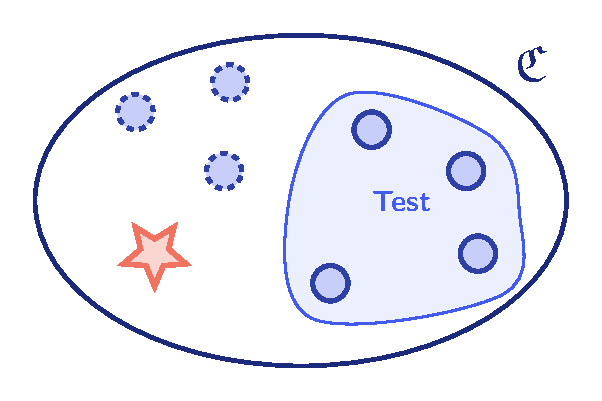
\includegraphics[width=\linewidth]{tikz-figures/canvas/blindness.pdf}
    \caption{Under a \textbf{blindness} protocol, the target computation is embedded in a class $\class$ containing the initial computation (red star) and classically simulable instances (blue circles), all indistinguishable when delegated. Those yielding deterministic measurement outcomes are named \emph{traps}.}
    \label{fig:verif-canvas:blindness}
  \end{subfigure}
  \hfill
  \begin{subfigure}[b]{0.45\linewidth}
    \centering
    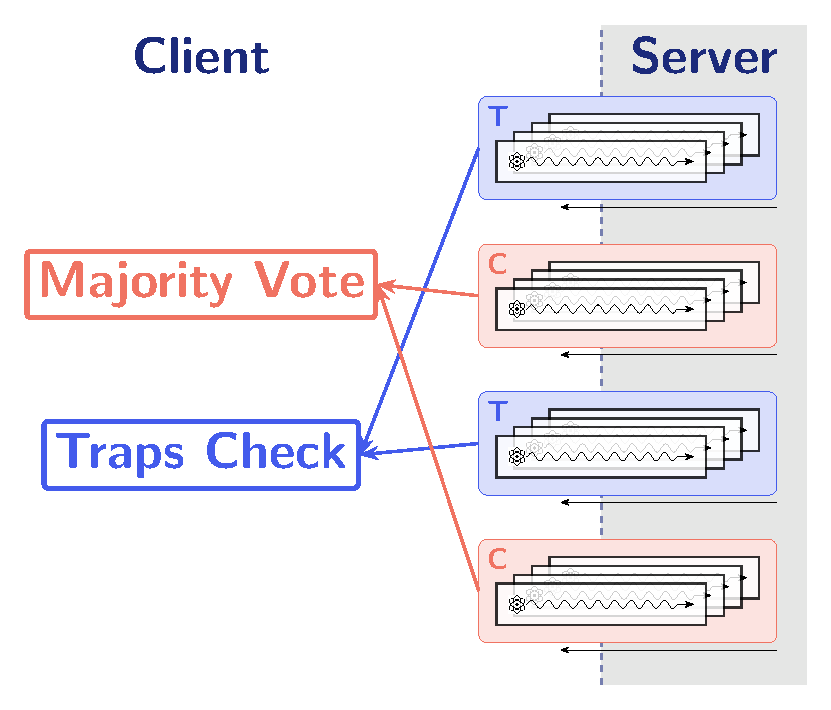
\includegraphics[width=\linewidth]{tikz-figures/canvas/verification.pdf}
    \caption{In the \textbf{Verification} protocol, test (blue boxes) and computation rounds (red boxes) are blindly delegated to the Server. Trap outcomes are checked by the Client to yield the acceptance/rejection decision; computation outcomes are aggregated via a majority vote.}
    \label{fig:verif-canvas:verification}
  \end{subfigure}
  \caption{The Test/Computation paradigm.}
  \label{fig:verif-canvas}
\end{figure}

Our work essentially introduces and formalizes constructions for the Test/Computation paradigm in the Clifford+MSI model. This representation captures both standard circuit-model architectures and the measurement-based implementations where qubits measured in a non-Pauli basis are instead prepared in a magic state and measured in an adaptive Pauli basis \cite{SDKO07direct}.

\subsubsection{Blindness (Section~\ref{section:blindness}).}
The Test/Computation paradigm does not require the computation to be entirely blinded when delegated: it only requires enough blindness to make the target computation indistinguishable from classically simulable computations that can then be used as tests.
The central idea is to exploit the fact that, in this model, the only potential source of computational non-classicality is carried by the injected qubits when they are in a magic state, while the surrounding Clifford structure is efficiently simulable and can be made public.
\paragraph{Blinding the Magic only.}
By hiding which single-qubit states are injected, the Client can make different computations indistinguishable to the Server: genuine quantum computations using magic states, and classically simulable test computations obtained by injecting only stabilizer states. This is formalized through a blindness concept that we call \emph{magic-blindness}, captured by Resource~\ref{informalresource:mblind_DQC}, that we present here informally.
\begin{informalresource}
    \caption{Magic-Blind DQC}
    \label{informalresource:mblind_DQC}
    \begin{algorithmic}[0]
        \State \textbf{Client's Inputs:} computation on $n$ qubits and $t$ ancillas.
        \State \textbf{Server's Inputs:} cheating bit $c\in\bin$, set to $0$ if honest.
        \State \textbf{Public Information:} Clifford parts of the computation.
        \Procedure{Computation by the Resource}{}
        \If{$c=0$ (honest behavior)}
        \State Resource performs the intended computation and measures the qubits
        \State Resource returns the classical bit-string of measurement outcomes to the Client.
        \Else{(malicious behavior)}
        \State Server provides a state and a CPTP map to perform, based on the public information only.
        \State Resource applies the CPTP map and returns the outcomes to the Client.
        \EndIf
        \EndProcedure
    \end{algorithmic}
\end{informalresource}
The Magic-Blind Delegated Quantum Computation Resource allows a Client to delegate a computation on $n$ qubits and $t$ ancillas, while hiding whether the injected ancillas are magic states, since only the content of the Clifford gates of the computation is leaked. By definition of this resource, any Server cheating behavior does not allow it to infer this information.
\begin{center}
    \textit{
        Magic-blindness is the ingredient that creates the indistinguishability required to embed efficiently simulable computations in the Clifford+MSI model.
    }
\end{center}

\paragraph{Composing Blind State Injection and Blind Measurements.}
The core idea of the protocol we present to realize this Resource is for the Client to apply a Pauli encryption to the states before sending them, thereby perfectly blinding their content through a quantum one-time pad, and to keep track of the evolution of the Pauli frame to later undo this encryption by decoding the measurement outcomes returned by the Server. Since all operations that the Server is supposed to apply are Clifford, this tracking is efficient. Intuitively, if the Server is not honest, it might return a bad result---we deal with this in the verification part---but it never learns the content of the state, which is what matters for our purposes.
\setcounter{informalprotocol}{3}
\begin{informalprotocol}
    \caption{Magic-Blind Delegated Quantum Computation}
    \label{informal:protocol:mblind_DQC}
    \begin{algorithmic}[0]
        \State Client sends an encrypted input state to the Server.
        \For{$i \le t$}
        \State Server applies public Clifford layer $\C_i$, and
        \State Client and Server perform a blind state-injection gadget.
        \Comment{Protocol~\ref{protocol:blind-gate}}
        \EndFor
        \State Server applies final Clifford $\C_{t+1}$ and measures all qubits, Client decodes. \Comment{Protocol~\ref{protocol:blind-meas}}
    \end{algorithmic}
\end{informalprotocol}

This protocol is built by composing sub-protocols, leveraging composability for its security. The first one makes the Server do a Clifford layer followed by a state injection, where all the qubits are blinded. It is used for as many layers as the computation has. Then a final Clifford layer followed by measurements, where all the qubits are again blinded. Those ideal behaviors are respectively implemented by a Blind State-Injection Protocol~\ref{protocol:blind-gate} and Blind Measurements Protocol~\ref{protocol:blind-meas}, all detailed in Section~\ref{section:blindness}.

\paragraph{Consequence: Clifford and non-Clifford delegated indistinguishably}
The main consequence of using the above protocol is what we aimed for: stabilizer states can be injected instead of magic states, and the computation becomes entirely Clifford on $n+t$ qubits, instead of the initial non-Clifford computation $C$ on $n$ qubits (tracing out the $t$ ancillas after they are injected). Throughout the work, when no magic states are injected, we refer to the resulting $n+t$-qubit Clifford as $\G$: it is the circuit obtained by interleaving the Clifford parts of the initial computation with $\CNOT$ on the ancillas to perform state injection. The same cannot be said when magic states are injected since conditioned Clifford operations need to be added to ensure that the state is being transformed correctly. Indeed, Magic-State Injection requires $\CNOT$, measurement, and conditioned Clifford to implement a $\T$-gate. When injecting a stabilizer state instead, the conditioned Clifford can be dropped, and the measurements can thus be delayed: the evolution of the entire system on $n+t$ qubits can be simulated classically and is described by the $n+t$-qubit Clifford circuit $\G$ (see Equation~\ref{eq:blindness:G} and Figure~\ref{fig:blindness:G}).

Ultimately, Magic-Blindness embeds the initial computation $C$ in a class $\class$ of computations that are delegated indistinguishably under Protocol~\ref{informal:protocol:mblind_DQC}: they all consist of the same Clifford parts, and differ by the states that are injected. The class $\class$ contains the initial computation $C$ as well as other instances that perform the Clifford $\G$ on stabilizer inputs.

\paragraph{Consequence on malicious behavior.}
Since Protocol~\ref{informal:protocol:mblind_DQC} is proven composably secure, \emph{i.e.}, it constructs Resource~\ref{informalresource:mblind_DQC}, any adversarial deviation is captured by a single strategy at the level of the resource. Magic-blindness then guarantees that all computations in the class are indistinguishable to the Server. Therefore, a malicious Server cannot condition its attack on a particular instance: the same deviation acts on every computation in the class, a property that will be crucial in the verification analysis.

\begin{center}
    \textit{
        Because the Server cannot distinguish instances in the class $\class$, any malicious deviation must act uniformly across all instances, including the target computation and the efficiently simulable ones used for tests.
    }
\end{center}

\subsubsection{Verification (Section~\ref{section:verification}).}

\paragraph{Leveraging Magic-Blindness}
We leverage the Magic-Blind DQC Protocol above to realize the ideal Verification Resource with Protocol~\ref{informal:protocol:verification} that follows the Test/Computation paradigm presented in Figure~\ref{fig:verif-canvas}. It interleaves test and computation rounds blindly using Protocol~\ref{informal:protocol:mblind_DQC}, where test rounds are instances of $\class$ that are efficiently simulable and yield deterministic measurement outcomes—\emph{traps}—allowing the Client to catch a cheating Server. This protocol is designed for $\BQP$ computations, for which the input is a classical bitstring and the output is a decision bit.

\setcounter{informalprotocol}{4}
\begin{informalprotocol}
    \caption{Verified Delegated Quantum Computation}
\label{informal:protocol:verification}
\begin{algorithmic}[0]
  \State \textbf{Client inputs:} quantum computation $C$, input bitstring $\x$, parameters $d, s, w$.

  \State Client chooses a random partition of $d$ computation and $s$ test rounds.
  \Comment{Private
  set-up}
  \State Client delegates the rounds blindly using Informal Protocol~\ref{informal:protocol:mblind_DQC}.
  \Comment{Blind delegation}

  \State If more than $w$ test rounds had trap failures, abort; else go to next step. \Comment{Traps check}
  \State If output $z$ has more than $d/2$ occurrences, output $z$ ; else $z\oplus 1$. \Comment{Majority vote}

\end{algorithmic}
\end{informalprotocol}

\paragraph{Designing traps for the Clifford+MSI model.}
Traps must be designed to detect any Server deviation that might harm the computation. However, in Section~\ref{subsection:blind:Pauli dev} we show that as a consequence of using MB-DQC at each round, which contains a Pauli encryption of the entire register on which the Server operates (potentially maliciously), any deviation with respect to the instructed behavior can be reduced to a convex combination of Pauli deviations, because of a Pauli Twirl. This yields a classification of Pauli deviations into \emph{harmful} (flipping at least one measurement outcome) and \emph{harmless} (not flipping any measurement outcome) deviations.

We use this to introduce, in Section~\ref{subsection:framework single qubit},
a way to detect any harmful deviation while being insensitive to harmless ones.
It is based on the following intuition: because deviations are only Pauli, they can only deterministically flip deterministic Pauli measurements. Hence we introduce the concept of \emph{traps} for Clifford+MSI computation: computations in $\class$ yielding efficiently simulable and deterministic measurement outcomes that can be used to check the presence of (harmful) deviations.
Intuitively, because such computations are described by the Clifford evolution $\G$, a trap can be obtained by injecting stabilizer states according to the following logic: in order to make the measurement of qubit $i$ deterministic, the output state must be stabilized by $\Z_i$, thus the input state must be stabilized by $\G^\dagger \Z_i\G$. Preparing a $+1$-eigenstate of this operator and injecting it to the computation, qubit by qubit, and checking outcome of qubit $i$, is thus a way to detect if a Pauli deviation was present on that qubit. Having one trap per output qubit is the construction we propose in Section~\ref{subsection:framework single qubit}, building a protocol on top of it in Section~\ref{subsection:verification:protocol} and proving its security. Later, in Section~\ref{subsection:framework generalized}, we show that this approach can be generalized into a more modular approach, building traps for subsets of qubits. This freedom to design traps while still detecting any harmful deviation is thus at the core of a verification framework in the Clifford+MSI model (depicted on Figure~\ref{fig:canvas-framework}).
\begin{figure}[h]
  \centering
  \begin{subfigure}[c]{0.40\linewidth}
    \centering
    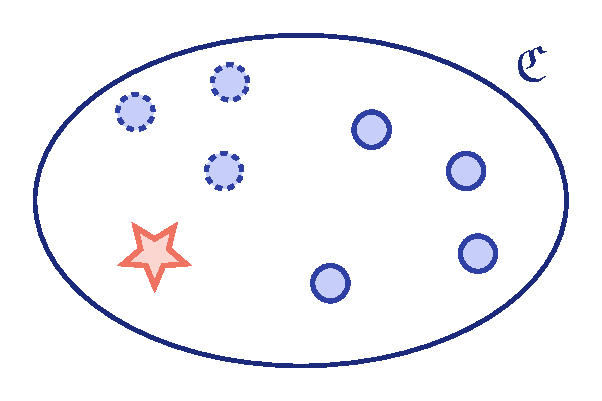
\includegraphics[width=\linewidth]{tikz-figures/canvas/blindness-modular.pdf}
    \caption{Blindness.}
    \label{fig:canvas-framework:blindness}
  \end{subfigure}
  \hfill
  \begin{subfigure}[c]{0.18\linewidth}
    \centering
    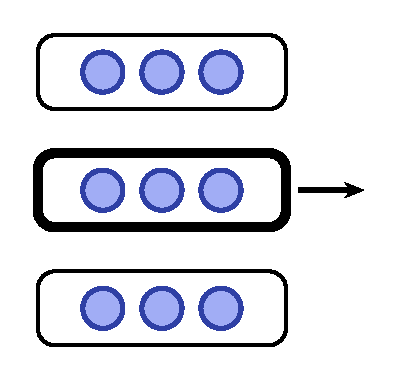
\includegraphics[width=\linewidth]{tikz-figures/canvas/traps-design.pdf}
    \caption{Trap design.}
    \label{fig:canvas-framework:traps}
  \end{subfigure}
  \hfill
  \begin{subfigure}[c]{0.38\linewidth}
    \centering
    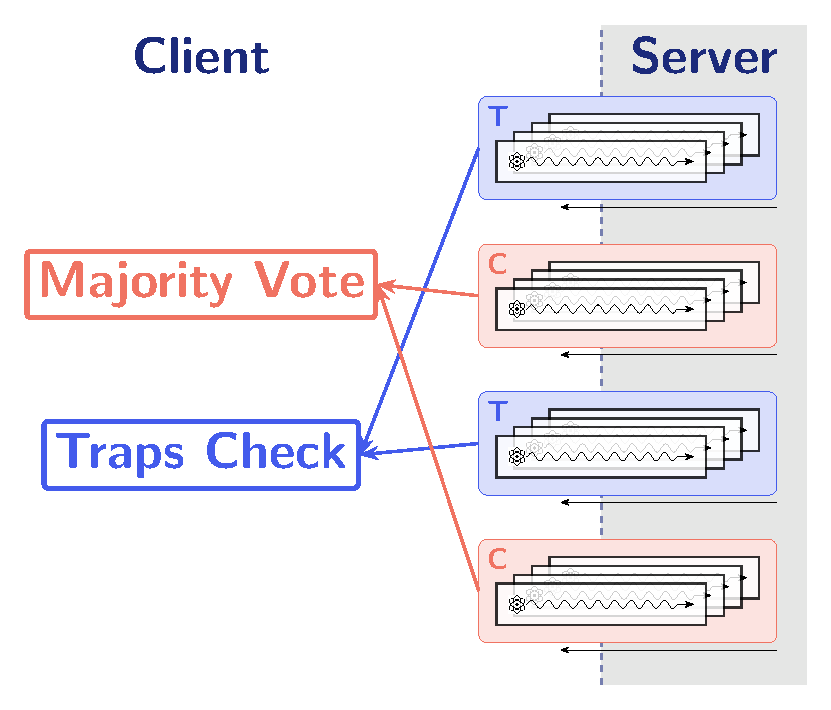
\includegraphics[width=\linewidth]{tikz-figures/canvas/verification.pdf}
    \caption{Verification.}
    \label{fig:canvas-framework:verification}
  \end{subfigure}
  \caption{\textbf{The modular trap-based verification framework.}
    \emph{(\subref{fig:canvas-framework:blindness}) Blindness.}
    Magic-blindness embeds the target computation $C$ in a class $\class$ containing it (denoted by a red star) alongside multiple families of efficiently simulable computations (blue circles), some of them yielding deterministic measurement outcomes (solid line)—those are named \emph{traps}.
    \emph{(\subref{fig:canvas-framework:traps}) Trap design.}
    The Client selects one trap family (highlighted row) from the available options; any family that detects all Server deviations suffices.
    \emph{(\subref{fig:canvas-framework:verification}) Verification.}
    Using the chosen family, the protocol proceeds exactly as in Figure~\ref{fig:verif-canvas:verification}: test and computation rounds are blindly delegated, trap outcomes are checked, and computation outcomes are aggregated by majority vote.}
  \label{fig:canvas-framework}
\end{figure}

\paragraph{Main result: efficient, composable, noise-robust verification in the circuit-model.}

\begin{itemize}
    \item \textbf{Composability:} we prove the composable security of Protocol~\ref{informal:protocol:verification}, \emph{i.e.}, we show that it implements Resource~\ref{informalresource: VDQC} up to a construction error $\epsilon$ that corresponds to the distinguishing probability between the Protocol and the Resource for any unbounded adversary.
    \item \textbf{Exponential security:} we show that in the presence of a malicious Server, $\epsilon$ corresponds to the maximum probability to trigger less than $w$ test rounds out of $s$ while corrupting more than $d/2$ computation rounds, enough to alter the outcome of the majority vote. In Lemma~\ref{lemma:security error}, we show that this quantity is negligible in $d, s$, as long as $w$ is chosen within a specific range depending on the number of types of tests and the BQP error of the computation. It thus shows that the security error decreases exponentially with the number of rounds involved in the protocol.
    \item \textbf{Noise-robustness:} we show that when the Server is honest but operates on a device with a circuit-level noise that affects all rounds with probability less than $p_{err}$,
    traps are not triggered as long as $p_{err}< w/s$. As a consequence, the level of noise that is tolerated depends on where the test rounds threshold is set, which depends on the desired security.
\end{itemize}

\begin{center}
    \textit{
        Magic-blindness creates an indistinguishable computation class; this class enables trap constructions that detect all deviations, yielding composable verified delegation with exponential security and correctness robust to circuit-level noise.
    }
\end{center}

\paragraph{Organization of the paper.} The rest of the paper is organized as follows. We start with preliminaries in Section~\ref{section:prelims}. In Section~\ref{section:blindness}, we present the constructions and results relevant for magic-blindness, and in Section~\ref{section:verification}, we show how to leverage this to build a composably secure verification protocol following the Test/Computation paradigm. Finally, we conclude in Section~\ref{section:Discussion}.
